\documentclass[11pt]{article}
\usepackage[margin=1in]{geometry}
\usepackage{enumitem}
\usepackage{amsmath}
\usepackage{amssymb}
\usepackage{xcolor}
\usepackage{tikz}
\usepackage{fancyhdr}
\usepackage{tcolorbox}
\tcbuselibrary{skins,breakable}
\usepackage{array}
\usepackage{booktabs}
\usepackage{multicol}

\definecolor{sectioncolor}{RGB}{85,105,20}
\definecolor{keygreen}{RGB}{200,240,200}

\pagestyle{fancy}
\fancyhf{}
\rhead{Community Ecology Quiz}
\lhead{Name: \underline{\hspace{3cm}}}
\rfoot{Page \thepage}

\title{\textbf{Community Ecology Comprehensive Practice Exam}}
\author{Study Guide for 100\% Success}
\date{}

\begin{document}
\maketitle
\thispagestyle{fancy}

\begin{tcolorbox}[colback=blue!5!white,colframe=blue!75!black,title=\textbf{Instructions}]
Answer all questions completely. Show your work where applicable. This exam covers all 12 Community Ecology topics:
(1) Interspecific interactions, (2) Ecological niche, (3) Intraspecific vs.\ interspecific competition,
(4) Competition avoidance, (5) Lotka-Volterra model, (6) Symbiotic interactions,
(7) Ecological succession, (8) Shannon-Weiner diversity index, (9) Biodiversity concepts,
(10) Predator-prey dynamics and mimicry, (11) Community equilibrium and trophic cascades,
(12) Eco-agriculture. Total: 380 points.
\end{tcolorbox}

\vspace{0.4cm}

%------------------------------------------------------------
\section*{Part A: Definitions and Concepts (2 pts each = 20 pts)}
%------------------------------------------------------------
Define each of the following terms clearly and concisely.

\begin{enumerate}[label=\textbf{\arabic*.}]
  \item \textbf{Interspecific interaction}: \underline{\hspace{10cm}}
        \vspace{0.5cm}
  \item \textbf{Ecological niche}: \underline{\hspace{10cm}}
        \vspace{0.5cm}
  \item \textbf{Fundamental niche}: \underline{\hspace{10cm}}
        \vspace{0.5cm}
  \item \textbf{Realized niche}: \underline{\hspace{10cm}}
        \vspace{0.5cm}
  \item \textbf{Competitive exclusion principle}: \underline{\hspace{9cm}}
        \vspace{0.5cm}
  \item \textbf{Resource partitioning}: \underline{\hspace{10cm}}
        \vspace{0.5cm}
  \item \textbf{Character displacement}: \underline{\hspace{10cm}}
        \vspace{0.5cm}
  \item \textbf{Mutualism}: \underline{\hspace{10cm}}
        \vspace{0.5cm}
  \item \textbf{Ecological succession}: \underline{\hspace{10cm}}
        \vspace{0.5cm}
  \item \textbf{Shannon-Weiner diversity index}: \underline{\hspace{9cm}}
        \vspace{0.5cm}
\end{enumerate}

\clearpage

%------------------------------------------------------------
\section*{Part B: Multiple Choice (2 pts each = 100 pts)}
%------------------------------------------------------------
Circle the best answer for each question.

\begin{enumerate}[label=\textbf{\arabic*.}]

\item Which interspecific interaction benefits one species while the other is unaffected?
\begin{enumerate}[label=\Alph*.]
  \item Mutualism
  \item Commensalism
  \item Parasitism
  \item Amensalism
\end{enumerate}

\item In the Lotka-Volterra competition model, species coexistence occurs when:
\begin{enumerate}[label=\Alph*.]
  \item intraspecific competition exceeds interspecific competition for both species
  \item interspecific competition exceeds intraspecific competition for both species
  \item one species always dominates
  \item carrying capacities are equal
\end{enumerate}

\item The Shannon-Weiner index $H = 0$ when:
\begin{enumerate}[label=\Alph*.]
  \item all species are equally abundant
  \item only one species is present
  \item species richness is highest
  \item evenness equals 1
\end{enumerate}

\item Which type of competition involves direct physical interference between organisms?
\begin{enumerate}[label=\Alph*.]
  \item Exploitative competition
  \item Scramble competition
  \item Interference competition
  \item Contest competition
\end{enumerate}

\item Primary succession begins on:
\begin{enumerate}[label=\Alph*.]
  \item abandoned agricultural fields
  \item bare rock with no soil
  \item burned forests
  \item flood plains
\end{enumerate}

\item Which is an example of Batesian mimicry?
\begin{enumerate}[label=\Alph*.]
  \item Two toxic species resembling each other
  \item A harmless species mimicking a toxic one
  \item A predator mimicking its prey
  \item Cryptic coloration in prey
\end{enumerate}

\item Keystone species are defined by:
\begin{enumerate}[label=\Alph*.]
  \item having the largest population in the community
  \item having a disproportionately large impact relative to their abundance
  \item being the most abundant species
  \item being at the top of the food chain
\end{enumerate}

\item Mycorrhizal associations between fungi and plant roots are examples of:
\begin{enumerate}[label=\Alph*.]
  \item parasitism
  \item commensalism
  \item mutualism
  \item amensalism
\end{enumerate}

\item The realized niche is:
\begin{enumerate}[label=\Alph*.]
  \item wider than the fundamental niche
  \item the niche in the absence of competition
  \item narrower than the fundamental niche due to biotic interactions
  \item identical to the fundamental niche
\end{enumerate}

\item In a $P > R$ community (production exceeds respiration):
\begin{enumerate}[label=\Alph*.]
  \item the community is in climax state
  \item organic matter is accumulating (biomass increasing)
  \item decomposition exceeds production
  \item the community is losing biodiversity
\end{enumerate}

\clearpage

\item Which succession type involves changes driven by the organisms themselves?
\begin{enumerate}[label=\Alph*.]
  \item Allogenic succession
  \item Primary succession
  \item Autogenic succession
  \item Secondary succession
\end{enumerate}

\item Resource partitioning reduces competition by:
\begin{enumerate}[label=\Alph*.]
  \item eliminating one competitor
  \item allowing species to use different resources or habitats
  \item increasing carrying capacity
  \item reducing population size
\end{enumerate}

\item Character displacement refers to:
\begin{enumerate}[label=\Alph*.]
  \item evolution of similar traits in allopatric species
  \item divergence of traits in sympatric competing species to reduce competition
  \item migration to new habitats
  \item loss of competitive ability
\end{enumerate}

\item Which coloration strategy warns predators of toxicity?
\begin{enumerate}[label=\Alph*.]
  \item Cryptic coloration
  \item Aposematic coloration
  \item Disruptive coloration
  \item Countershading
\end{enumerate}

\item The trophic cascade concept describes:
\begin{enumerate}[label=\Alph*.]
  \item energy flow from producers to consumers
  \item indirect effects of predators on lower trophic levels
  \item nutrient cycling in ecosystems
  \item primary productivity rates
\end{enumerate}

\item In the lynx-hare cycle, hare populations decline because:
\begin{enumerate}[label=\Alph*.]
  \item disease outbreaks
  \item lynx predation reduces hare numbers, then lynx starve
  \item resource depletion alone
  \item competition from other herbivores
\end{enumerate}

\item Nitrogen-fixing nodules on legume roots involve:
\begin{enumerate}[label=\Alph*.]
  \item mycorrhizal fungi
  \item \textit{Rhizobium} bacteria
  \item cyanobacteria in soil
  \item \textit{Azotobacter} fungi
\end{enumerate}

\item Which eco-agricultural practice involves growing multiple crop species simultaneously?
\begin{enumerate}[label=\Alph*.]
  \item Crop rotation
  \item Monoculture
  \item Intercropping
  \item No-tillage
\end{enumerate}

\item Competitive exclusion principle states that:
\begin{enumerate}[label=\Alph*.]
  \item two species can coexist if they partition resources
  \item two species competing for identical resources cannot coexist indefinitely
  \item competition always leads to extinction
  \item stronger species always outcompetes weaker ones
\end{enumerate}

\item Ecological engineers modify:
\begin{enumerate}[label=\Alph*.]
  \item their own physiology in response to stress
  \item the physical environment, creating habitat for other species
  \item their diet based on available prey
  \item population growth rate
\end{enumerate}

\clearpage

\item Which interspecific interaction harms both species involved?
\begin{enumerate}[label=\Alph*.]
  \item Mutualism ($+/+$)
  \item Commensalism ($+/0$)
  \item Competition ($-/-$)
  \item Parasitism ($+/-$)
\end{enumerate}

\item The pioneer community in primary succession on bare rock typically consists of:
\begin{enumerate}[label=\Alph*.]
  \item grasses and shrubs
  \item lichens and mosses
  \item coniferous trees
  \item deciduous forest
\end{enumerate}

\item A dominant species in a community is characterized by:
\begin{enumerate}[label=\Alph*.]
  \item highest biomass or abundance
  \item greatest impact per individual
  \item most unique ecological role
  \item largest body size
\end{enumerate}

\item Top-down control in a community occurs when:
\begin{enumerate}[label=\Alph*.]
  \item primary productivity limits herbivore populations
  \item predators regulate prey and lower trophic levels
  \item nutrients limit plant growth
  \item decomposers control nutrient availability
\end{enumerate}

\item M\"{u}llerian mimicry involves:
\begin{enumerate}[label=\Alph*.]
  \item a harmless species mimicking a toxic one
  \item two or more toxic/unpalatable species resembling each other
  \item prey mimicking predators
  \item camouflage in vegetation
\end{enumerate}

\item The fundamental niche includes:
\begin{enumerate}[label=\Alph*.]
  \item only the resources actually used by a species
  \item all conditions under which a species can potentially survive and reproduce
  \item the narrowed niche due to competition
  \item the niche shared with another species
\end{enumerate}

\item Scramble competition results in:
\begin{enumerate}[label=\Alph*.]
  \item one winner taking all resources
  \item all competing individuals receiving insufficient resources
  \item resource partitioning
  \item character displacement
\end{enumerate}

\item Which of the following is an example of amensalism?
\begin{enumerate}[label=\Alph*.]
  \item A bird eating insects flushed by cattle
  \item A tree shading and suppressing undergrowth plants
  \item Two herbivores eating the same grass
  \item Ants protecting aphids
\end{enumerate}

\item In secondary succession, the process is faster than primary succession because:
\begin{enumerate}[label=\Alph*.]
  \item more species are available as colonizers
  \item soil and seed banks are already present
  \item disturbance is more severe
  \item competition is lower
\end{enumerate}

\item Protocooperation differs from mutualism in that:
\begin{enumerate}[label=\Alph*.]
  \item both species benefit more in protocooperation
  \item the interaction in protocooperation is not obligatory
  \item protocooperation involves more species
  \item protocooperation only benefits one species
\end{enumerate}

\clearpage

\item The grey wolf reintroduction in Yellowstone demonstrated:
\begin{enumerate}[label=\Alph*.]
  \item competitive exclusion of elk
  \item a trophic cascade affecting vegetation and river morphology
  \item mutualism between wolves and ravens
  \item primary succession on riverbanks
\end{enumerate}

\item Dead mulch in eco-agriculture refers to:
\begin{enumerate}[label=\Alph*.]
  \item living cover crops left in the field
  \item dried organic matter covering soil surface
  \item crop residues ploughed under
  \item green manure from legumes
\end{enumerate}

\item Which index value indicates maximum evenness in a 3-species community?
\begin{enumerate}[label=\Alph*.]
  \item $H = 0$
  \item $H = \ln(3)$
  \item $H = 1$
  \item $H = 3$
\end{enumerate}

\item Mertensian mimicry involves:
\begin{enumerate}[label=\Alph*.]
  \item harmless species mimicking toxic ones
  \item a deadly species mimicking a moderately toxic model so predators can learn
  \item two toxic species with similar warning coloration
  \item countershading in aquatic species
\end{enumerate}

\item Intraspecific competition occurs between:
\begin{enumerate}[label=\Alph*.]
  \item different species competing for the same resource
  \item individuals of the same species
  \item predators and their prey
  \item parasites and hosts
\end{enumerate}

\item Which abiotic factor could determine the fundamental niche of a cold-water fish species?
\begin{enumerate}[label=\Alph*.]
  \item Presence of competing species
  \item Predator distribution
  \item Water temperature range
  \item Parasites
\end{enumerate}

\item Agroforestry integrates:
\begin{enumerate}[label=\Alph*.]
  \item only annual crops
  \item trees with crops or livestock
  \item monocultures with irrigation
  \item synthetic fertilizers with tillage
\end{enumerate}

\item In the Lotka-Volterra model, if species A's isocline lies above species B's isocline, then:
\begin{enumerate}[label=\Alph*.]
  \item species B will always win
  \item species A will always win
  \item coexistence is stable
  \item both species go extinct
\end{enumerate}

\item A lichen is an example of:
\begin{enumerate}[label=\Alph*.]
  \item parasitism between algae and fungi
  \item mutualism between algae/cyanobacteria and fungi
  \item commensalism
  \item competition
\end{enumerate}

\item Bottom-up control refers to:
\begin{enumerate}[label=\Alph*.]
  \item predator limitation of prey
  \item nutrient or primary productivity limitation propagating up the food web
  \item decomposer control of producers
  \item top predator control
\end{enumerate}

\clearpage

\item Which succession leads to a climax community with $P \approx R$?
\begin{enumerate}[label=\Alph*.]
  \item Only primary succession
  \item Both primary and secondary succession converge toward climax
  \item Only secondary succession
  \item Microsuccession
\end{enumerate}

\item Contest competition results in:
\begin{enumerate}[label=\Alph*.]
  \item all individuals sharing equally
  \item some individuals obtaining full resource needs while others obtain none
  \item character displacement
  \item resource partitioning
\end{enumerate}

\item Which is NOT a defense mechanism against predation?
\begin{enumerate}[label=\Alph*.]
  \item Thorns (mechanical defense)
  \item Toxins (chemical defense)
  \item Aposematic coloration
  \item Protocooperation
\end{enumerate}

\item Minimum tillage practices in eco-agriculture help by:
\begin{enumerate}[label=\Alph*.]
  \item increasing soil compaction
  \item reducing soil disturbance, preserving soil structure and biodiversity
  \item eliminating all weeds
  \item requiring more fertilizer
\end{enumerate}

\item Crop rotation helps in eco-agriculture by:
\begin{enumerate}[label=\Alph*.]
  \item reducing crop diversity
  \item breaking pest and disease cycles and improving soil fertility
  \item increasing herbicide use
  \item requiring more water
\end{enumerate}

\item Serule refers to:
\begin{enumerate}[label=\Alph*.]
  \item a climax community
  \item a microsuccession sequence in a small habitat patch
  \item a pioneer community
  \item allogenic succession
\end{enumerate}

\item Which type of niche concept considers evolutionary history of the species?
\begin{enumerate}[label=\Alph*.]
  \item Fundamental niche
  \item Realized niche
  \item Evolutionary niche
  \item Ecological niche
\end{enumerate}

\item Species richness refers to:
\begin{enumerate}[label=\Alph*.]
  \item the relative abundance of each species
  \item the total number of species in a community
  \item the $H$ value of Shannon index
  \item the biomass of dominant species
\end{enumerate}

\item Predator-prey cycling in the Lotka-Volterra predation model shows:
\begin{enumerate}[label=\Alph*.]
  \item stable equilibrium with no oscillation
  \item oscillating populations with prey peak preceding predator peak
  \item prey going extinct first
  \item predator going extinct first
\end{enumerate}

\item Which statement about high-biodiversity communities is correct?
\begin{enumerate}[label=\Alph*.]
  \item They are less stable than low-diversity communities
  \item They tend to be more resistant and resilient to disturbances
  \item They have fewer ecological interactions
  \item They require more energy input
\end{enumerate}

\end{enumerate}

\clearpage

%------------------------------------------------------------
\section*{Part C: Fill in the Blank (2 pts each = 40 pts)}
%------------------------------------------------------------
Complete each statement with the correct term or phrase.

\begin{enumerate}[label=\textbf{\arabic*.}]
  \item The interspecific interaction where one species benefits and the other is harmed is called \underline{\hspace{3cm}}.
  \item The \underline{\hspace{3cm}} niche represents all conditions under which a species can survive in the absence of competitors.
  \item When two species with identical niches compete, the \underline{\hspace{3cm}} principle predicts one will be excluded.
  \item The formula for the Shannon-Weiner index is $H = -\sum p_i$ \underline{\hspace{2cm}} $p_i$.
  \item In primary succession, the first colonizers are called \underline{\hspace{3cm}} species.
  \item Batesian mimicry involves a \underline{\hspace{3cm}} species resembling a toxic one.
  \item Resource use differences that reduce competition between species is called \underline{\hspace{3cm}}.
  \item Wolves, sea otters, and starfish are examples of \underline{\hspace{3cm}} species.
  \item The reintroduction of grey wolves in Yellowstone demonstrated a \underline{\hspace{3cm}} cascade.
  \item In eco-agriculture, \underline{\hspace{3cm}} involves growing tree species with crops or livestock.
  \item The mutualistic association between fungi and plant roots is called \underline{\hspace{3cm}}.
  \item When production exceeds respiration in a community ($P > R$), \underline{\hspace{3cm}} is accumulating.
  \item \underline{\hspace{3cm}} succession occurs on previously disturbed land that still has soil.
  \item The evolutionary divergence of traits in sympatric competing species is called \underline{\hspace{3cm}}.
  \item Two toxic species resembling each other is called \underline{\hspace{3cm}} mimicry.
  \item In the Lotka-Volterra model, coexistence requires that \underline{\hspace{2.5cm}} competition is stronger than \underline{\hspace{2.5cm}} competition for both species.
  \item The interspecific interaction where one species benefits and the other is unaffected is called \underline{\hspace{3cm}}.
  \item Dead organic matter used as soil cover in eco-agriculture is called \underline{\hspace{3cm}}.
  \item \underline{\hspace{3cm}} coloration warns predators of a prey's toxicity.
  \item A species that disproportionately shapes its community relative to its abundance is a \underline{\hspace{3cm}} species.
\end{enumerate}

\clearpage

%------------------------------------------------------------
\section*{Part D: Short Answer (5 pts each = 40 pts)}
%------------------------------------------------------------

\begin{enumerate}[label=\textbf{\arabic*.}]
  \item Describe the difference between interference competition and exploitative competition. Give one example of each.
  \vspace{2cm}

  \item Explain the concept of niche partitioning and how it allows species coexistence. Give a real-world example.
  \vspace{2cm}

  \item Describe the process of primary succession from bare rock to climax community. What happens to the $P\!:\!R$ ratio as succession proceeds?
  \vspace{2cm}

  \item Compare Batesian and M\"{u}llerian mimicry. What selective pressures maintain each system?
  \vspace{2cm}

  \item Explain what a trophic cascade is. Use the grey wolf reintroduction in Yellowstone as an example to describe both top-down and bottom-up control.
  \vspace{2cm}

  \item What is the Shannon-Weiner diversity index? Explain how a community can have high species richness but low $H$ value.
  \vspace{2cm}

  \item Describe three eco-agricultural practices and explain how each contributes to sustainable agriculture.
  \vspace{2cm}

  \item Compare autogenic and allogenic succession. Give one example of each type.
  \vspace{2cm}
\end{enumerate}

\clearpage

%------------------------------------------------------------
\section*{Part E: Matching (2 pts each = 20 pts)}
%------------------------------------------------------------
Match each term in Column A with its correct description in Column B. Write the correct letter in the blank.

\vspace{0.3cm}
\begin{tabular}{p{0.45\textwidth} p{0.05\textwidth} p{0.45\textwidth}}
\toprule
\textbf{Column A} & & \textbf{Column B} \\
\midrule
\textbf{1.} Mutualism & \underline{\phantom{XX}} & \textbf{a.} Indirect effects of predators rippling through trophic levels \\[0.3cm]
\textbf{2.} Competitive exclusion & \underline{\phantom{XX}} & \textbf{b.} Warning coloration advertising toxicity to predators \\[0.3cm]
\textbf{3.} Keystone species & \underline{\phantom{XX}} & \textbf{c.} Succession beginning on bare substrate without soil \\[0.3cm]
\textbf{4.} Aposematic coloration & \underline{\phantom{XX}} & \textbf{d.} Both species benefit but the interaction is not obligatory \\[0.3cm]
\textbf{5.} Realized niche & \underline{\phantom{XX}} & \textbf{e.} Measure of community diversity accounting for richness and evenness \\[0.3cm]
\textbf{6.} Trophic cascade & \underline{\phantom{XX}} & \textbf{f.} Both species benefit and the interaction is obligatory \\[0.3cm]
\textbf{7.} Character displacement & \underline{\phantom{XX}} & \textbf{g.} The niche space actually occupied due to biotic interactions \\[0.3cm]
\textbf{8.} Primary succession & \underline{\phantom{XX}} & \textbf{h.} Evolutionary trait divergence reducing competition between sympatric species \\[0.3cm]
\textbf{9.} Shannon-Weiner index & \underline{\phantom{XX}} & \textbf{i.} Species with disproportionate impact on community structure \\[0.3cm]
\textbf{10.} Protocooperation & \underline{\phantom{XX}} & \textbf{j.} Two species with identical niches cannot stably coexist \\[0.3cm]
\bottomrule
\end{tabular}

\clearpage

%------------------------------------------------------------
\section*{Part F: True or False (2 pts each = 30 pts)}
%------------------------------------------------------------
Write \textbf{T} (True) or \textbf{F} (False) on the line provided.

\begin{enumerate}[label=\textbf{\arabic*.}]
  \item \textbf{T / F} \underline{\phantom{XX}} The realized niche is always smaller than or equal to the fundamental niche.
  \item \textbf{T / F} \underline{\phantom{XX}} Commensalism benefits both interacting species.
  \item \textbf{T / F} \underline{\phantom{XX}} In M\"{u}llerian mimicry, all mimics are genuinely toxic or unpalatable.
  \item \textbf{T / F} \underline{\phantom{XX}} Primary succession is generally slower than secondary succession.
  \item \textbf{T / F} \underline{\phantom{XX}} Shannon-Weiner index $H$ increases when a community has lower evenness.
  \item \textbf{T / F} \underline{\phantom{XX}} Resource partitioning can reduce interspecific competition.
  \item \textbf{T / F} \underline{\phantom{XX}} Keystone species are always the most abundant species in a community.
  \item \textbf{T / F} \underline{\phantom{XX}} The grey wolf reintroduction in Yellowstone changed river morphology via trophic cascade.
  \item \textbf{T / F} \underline{\phantom{XX}} Intraspecific competition is generally less intense than interspecific competition for closely related species.
  \item \textbf{T / F} \underline{\phantom{XX}} Mycorrhizae benefit both the plant (improved nutrient uptake) and the fungus (carbohydrates).
  \item \textbf{T / F} \underline{\phantom{XX}} Agroforestry can increase biodiversity on farmland.
  \item \textbf{T / F} \underline{\phantom{XX}} The competitive exclusion principle states that competing species always coexist.
  \item \textbf{T / F} \underline{\phantom{XX}} In autogenic succession, the organisms themselves drive the changes in community composition.
  \item \textbf{T / F} \underline{\phantom{XX}} A higher $H$ value indicates greater biodiversity.
  \item \textbf{T / F} \underline{\phantom{XX}} Cryptic coloration is a form of chemical defense.
\end{enumerate}

\clearpage

%------------------------------------------------------------
\section*{Part G: Diagram Analysis (10 pts each = 30 pts)}
%------------------------------------------------------------

\subsection*{G1: Interspecific Interactions Table (10 pts)}
Complete the table below by filling in the effect on each species ($+$, $-$, or $0$) and providing one example for each interaction type.

\vspace{0.3cm}
\begin{tabular}{>{\bfseries}p{3.5cm} p{2.5cm} p{2.5cm} p{5cm}}
\toprule
\textbf{Interaction Type} & \textbf{Effect on Sp.\ A} & \textbf{Effect on Sp.\ B} & \textbf{Example} \\
\midrule
Competition & & & \\[0.8cm]
Predation/Antagonism & & & \\[0.8cm]
Parasitism & & & \\[0.8cm]
Commensalism & & & \\[0.8cm]
Mutualism & & & \\[0.8cm]
Amensalism & & & \\[0.8cm]
Neutralism & & & \\[0.8cm]
Protocooperation & & & \\[0.5cm]
\bottomrule
\end{tabular}

\vspace{0.5cm}

\subsection*{G2: Succession Diagram (10 pts)}
The diagram below represents a succession sequence. Use it to answer the questions.

\vspace{0.3cm}
\begin{center}
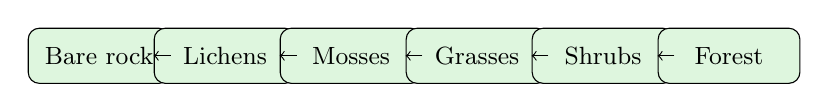
\begin{tikzpicture}[node distance=1.6cm, auto,
  every node/.style={rectangle, draw, rounded corners, fill=keygreen!60,
  minimum width=1.8cm, minimum height=0.7cm, font=\small}]
  \node (A) {Bare rock};
  \node (B) [right of=A] {Lichens};
  \node (C) [right of=B] {Mosses};
  \node (D) [right of=C] {Grasses};
  \node (E) [right of=D] {Shrubs};
  \node (F) [right of=E] {Forest};
  \draw[->] (A) -- (B);
  \draw[->] (B) -- (C);
  \draw[->] (C) -- (D);
  \draw[->] (D) -- (E);
  \draw[->] (E) -- (F);
\end{tikzpicture}
\end{center}

\begin{enumerate}[label=\alph*.]
  \item What are the pioneer species in this succession sequence, and why are they able to colonise bare rock?
  \vspace{1.5cm}
  \item How does the $P\!:\!R$ ratio change from bare rock to mature forest? What does this indicate about organic matter?
  \vspace{1.5cm}
  \item Is this an example of autogenic or allogenic succession? Explain your answer.
  \vspace{1.5cm}
\end{enumerate}

\subsection*{G3: Shannon-Weiner Diversity Calculation (10 pts)}

A researcher surveys a forest plot and records the following data:

\vspace{0.3cm}
\begin{center}
\begin{tabular}{lccc}
\toprule
\textbf{Species} & \textbf{Count ($n_i$)} & \textbf{Proportion ($p_i$)} & \textbf{$p_i \ln p_i$} \\
\midrule
Species A & 50 & 0.50 & \underline{\hspace{2cm}} \\
Species B & 30 & 0.30 & \underline{\hspace{2cm}} \\
Species C & 15 & 0.15 & \underline{\hspace{2cm}} \\
Species D &  5 & 0.05 & \underline{\hspace{2cm}} \\
\midrule
\textbf{Total} & \textbf{100} & \textbf{1.00} & \\
\bottomrule
\end{tabular}
\end{center}

\vspace{0.3cm}
\begin{enumerate}[label=\alph*.]
  \item Calculate $H = -\sum p_i \ln p_i$ for this community. Show all work.
  \vspace{2cm}
  \item Which species is the dominant species in this community? Justify your answer.
  \vspace{1cm}
  \item Interpret the $H$ value: does this community have high or low diversity? What would a perfectly even community of 4 species have as its maximum $H$?
  \vspace{1.5cm}
\end{enumerate}

\clearpage

%------------------------------------------------------------
\section*{Part H: Comparison Questions (10 pts each = 40 pts)}
%------------------------------------------------------------

\begin{enumerate}[label=\textbf{\arabic*.}]
  \item Compare the fundamental niche and the realized niche. In your answer, explain what factors cause them to differ and give an example.
  \vspace{3cm}

  \item Compare primary and secondary succession. Include differences in: (a) starting conditions, (b) typical pioneer species, (c) speed of succession, (d) $P\!:\!R$ ratio changes.
  \vspace{3cm}

  \item Compare intraspecific and interspecific competition. Which is typically more intense and why? How do organisms reduce the negative effects of each?
  \vspace{3cm}

  \item Compare Batesian and M\"{u}llerian mimicry. Which provides stronger protection and why? Give one example of each.
  \vspace{3cm}
\end{enumerate}

\clearpage

%------------------------------------------------------------
\section*{Part I: Application Problems (10 pts each = 30 pts)}
%------------------------------------------------------------

\subsection*{I1: Shannon-Weiner Calculation}
A researcher surveys two forest plots. Plot~1 has 3 species with 60, 30, and 10 individuals respectively. Plot~2 has 3 species with 34, 33, and 33 individuals respectively. Calculate $H$ for each plot, compare the results, and explain why they differ despite having the same species richness. Show all work.
\vspace{5cm}

\subsection*{I2: Lotka-Volterra Competition}
Two plant species A and B compete for light. Given:
\begin{itemize}
  \item $K_A = 200$,\quad $K_B = 150$
  \item $\alpha$ (effect of B on A) $= 0.8$
  \item $\beta$ (effect of A on B) $= 1.2$
\end{itemize}
Determine: (a) the zero-growth isocline for each species, (b) which species will win competitive exclusion, and (c) under what conditions coexistence would be possible.
\vspace{5cm}

\subsection*{I3: Trophic Cascade Analysis}
In a lake ecosystem: large fish eat small fish, small fish eat zooplankton, zooplankton eat phytoplankton. When large fish are removed by overfishing: (a) trace the expected changes through each trophic level, (b) identify whether this is a top-down or bottom-up effect, (c) predict what would happen to water clarity, (d) describe how reintroducing large fish might restore the system.
\vspace{5cm}

\clearpage

%------------------------------------------------------------
\section*{Part J: Essay Questions (15 pts each = 30 pts)}
%------------------------------------------------------------

\begin{enumerate}[label=\textbf{\arabic*.}]
  \item Describe the process of ecological succession from pioneer community to climax community, using either a terrestrial (bare rock $\rightarrow$ forest) or aquatic (open water $\rightarrow$ bog) example. In your answer, explain: (a) the role of pioneer and intermediate species in facilitating succession, (b) how the $P\!:\!R$ ratio changes from early to late succession, (c) the difference between autogenic and allogenic succession, (d) what a climax community is and whether it is truly stable.
  \vspace{5cm}

  \item Explain how keystone species and ecological engineers maintain community equilibrium and biodiversity. Use at least two specific examples. In your answer, discuss: (a) how keystone species differ from dominant species, (b) the role of trophic cascades, (c) how the removal of a keystone species affects community structure (with reference to the sea otter or grey wolf example), (d) what constitutes high vs.\ low biodiversity and why it matters.
  \vspace{5cm}
\end{enumerate}

\clearpage

%============================================================
% ANSWER KEY
%============================================================

\begin{tcolorbox}[enhanced,colback=green!20,colframe=green!60!black,
  arc=6pt,boxrule=1.2pt,title=\textbf{\large Answer Key --- Part A: Definitions},
  fonttitle=\bfseries,coltitle=black,breakable]
\begin{enumerate}[label=\textbf{\arabic*.},leftmargin=*]
  \item \textbf{Interspecific interaction}: Any relationship between individuals of different species (e.g., competition, predation, mutualism).
  \item \textbf{Ecological niche}: The multidimensional space of all biotic and abiotic conditions a species can tolerate and resources it uses.
  \item \textbf{Fundamental niche}: The full range of conditions a species can occupy in the absence of biotic interactions (competitors, predators, parasites).
  \item \textbf{Realized niche}: The actual niche a species occupies after accounting for biotic interactions; always $\leq$ fundamental niche.
  \item \textbf{Competitive exclusion principle}: Two species competing for identical limited resources cannot coexist indefinitely; one will be excluded.
  \item \textbf{Resource partitioning}: Differentiation in resource use (time, space, food type) among competing species, reducing interspecific competition.
  \item \textbf{Character displacement}: Evolutionary divergence of phenotypic traits (e.g., beak size) in sympatric competing species, reducing niche overlap.
  \item \textbf{Mutualism}: Obligatory interaction benefiting both species ($+/+$), e.g., mycorrhizae, nitrogen-fixing nodules, lichens.
  \item \textbf{Ecological succession}: Directional, sequential change in community composition over time following disturbance or on new substrate.
  \item \textbf{Shannon-Weiner diversity index}: $H = -\sum p_i \ln p_i$; quantifies diversity by incorporating species richness and evenness.
\end{enumerate}
\end{tcolorbox}

\vspace{0.4cm}

\begin{tcolorbox}[enhanced,colback=green!20,colframe=green!60!black,
  arc=6pt,boxrule=1.2pt,title=\textbf{\large Answer Key --- Part B: Multiple Choice},
  fonttitle=\bfseries,coltitle=black,breakable]
\begin{multicols}{5}
\begin{enumerate}[label=\textbf{\arabic*.},leftmargin=*,noitemsep]
  \item B \item A \item B \item C \item B
  \item B \item B \item C \item C \item B
  \item C \item B \item B \item B \item B
  \item B \item B \item C \item B \item B
  \item C \item B \item A \item B \item B
  \item B \item B \item B \item B \item B
  \item B \item B \item B \item B \item B
  \item C \item B \item B \item B \item B
  \item B \item B \item D \item B \item B
  \item B \item C \item B \item B \item B
\end{enumerate}
\end{multicols}
\end{tcolorbox}

\vspace{0.4cm}

\begin{tcolorbox}[enhanced,colback=green!20,colframe=green!60!black,
  arc=6pt,boxrule=1.2pt,title=\textbf{\large Answer Key --- Part C: Fill in the Blank},
  fonttitle=\bfseries,coltitle=black,breakable]
\begin{enumerate}[label=\textbf{\arabic*.},leftmargin=*]
  \item parasitism \item fundamental \item competitive exclusion \item $\ln$ \item pioneer
  \item harmless (palatable) \item resource partitioning \item keystone \item trophic \item agroforestry
  \item mycorrhiza \item biomass / organic matter \item Secondary \item character displacement \item M\"{u}llerian
  \item intraspecific / interspecific \item commensalism \item dead mulch \item Aposematic \item keystone
\end{enumerate}
\end{tcolorbox}

\vspace{0.4cm}

\begin{tcolorbox}[enhanced,colback=green!20,colframe=green!60!black,
  arc=6pt,boxrule=1.2pt,title=\textbf{\large Answer Key --- Part E: Matching},
  fonttitle=\bfseries,coltitle=black,breakable]
1--f, \quad 2--j, \quad 3--i, \quad 4--b, \quad 5--g, \quad 6--a, \quad 7--h, \quad 8--c, \quad 9--e, \quad 10--d
\end{tcolorbox}

\vspace{0.4cm}

\begin{tcolorbox}[enhanced,colback=green!20,colframe=green!60!black,
  arc=6pt,boxrule=1.2pt,title=\textbf{\large Answer Key --- Part F: True or False},
  fonttitle=\bfseries,coltitle=black,breakable]
1--T, \quad 2--F, \quad 3--T, \quad 4--T, \quad 5--F, \quad 6--T, \quad 7--F, \quad 8--T, \quad 9--F, \quad 10--T, \quad 11--T, \quad 12--F, \quad 13--T, \quad 14--T, \quad 15--F
\end{tcolorbox}

\vspace{0.4cm}

\begin{tcolorbox}[enhanced,colback=green!20,colframe=green!60!black,
  arc=6pt,boxrule=1.2pt,title=\textbf{\large Answer Key --- Part G3: Shannon-Weiner Calculation},
  fonttitle=\bfseries,coltitle=black,breakable]
$p_i \ln p_i$ values:
\begin{itemize}[noitemsep]
  \item Species A: $0.50 \times \ln(0.50) = 0.50 \times (-0.693) = -0.347$
  \item Species B: $0.30 \times \ln(0.30) = 0.30 \times (-1.204) = -0.361$
  \item Species C: $0.15 \times \ln(0.15) = 0.15 \times (-1.897) = -0.285$
  \item Species D: $0.05 \times \ln(0.05) = 0.05 \times (-2.996) = -0.150$
\end{itemize}
$H = -(-0.347 - 0.361 - 0.285 - 0.150) = \mathbf{1.143}$

Dominant species: \textbf{Species A} (50\% of individuals). Maximum $H$ for 4 equal species $= \ln(4) \approx 1.386$.
\end{tcolorbox}

\vspace{0.4cm}

\begin{tcolorbox}[enhanced,colback=green!20,colframe=green!60!black,
  arc=6pt,boxrule=1.2pt,title=\textbf{\large Answer Key --- Part I1: Shannon-Weiner},
  fonttitle=\bfseries,coltitle=black,breakable]
\textbf{Plot 1} ($N=100$; $n_1=60, n_2=30, n_3=10$):
$p_1=0.60,\ p_2=0.30,\ p_3=0.10$
$H = -(0.60\ln 0.60 + 0.30\ln 0.30 + 0.10\ln 0.10)$
$= -(0.60\times(-0.511) + 0.30\times(-1.204) + 0.10\times(-2.303))$
$= -(-0.306 - 0.361 - 0.230) = \mathbf{0.897}$

\textbf{Plot 2} ($N=100$; $n_1=34, n_2=33, n_3=33$):
$p_1 \approx p_2 \approx p_3 \approx 0.333$
$H = -3\times(0.333\ln 0.333) = -3\times(0.333\times(-1.099)) = -3\times(-0.366) = \mathbf{1.099} \approx \ln(3)$

\textbf{Conclusion}: Plot~2 has higher $H$ due to greater \textit{evenness}, despite both plots having the same species richness ($S=3$).
\end{tcolorbox}

\clearpage

%============================================================
% QUICK REFERENCE STUDY SHEET
%============================================================

\begin{tcolorbox}[enhanced,colback=olive!8,colframe=olive!70!black,
  arc=6pt,boxrule=1.4pt,halign=center,top=0.4cm,bottom=0.3cm]
  {\large\bfseries\color{sectioncolor} Quick Reference Study Sheet --- Community Ecology}
\end{tcolorbox}

\vspace{0.3cm}

\begin{multicols}{2}

\textbf{\color{sectioncolor}Key Formulas}

Shannon-Weiner Index:
\[ H = -\sum_{i=1}^{S} p_i \ln p_i \]
where $p_i = n_i / N$ (proportion of species $i$).
Maximum $H = \ln(S)$ (perfect evenness).

\vspace{0.2cm}

Lotka-Volterra Competition (zero-growth isoclines):
\[ \frac{dN_A}{dt}=0 \Rightarrow N_A = K_A - \alpha N_B \]
\[ \frac{dN_B}{dt}=0 \Rightarrow N_B = K_B - \beta N_A \]
Coexistence: intraspecific $>$ interspecific for both species.

\vspace{0.3cm}

\textbf{\color{sectioncolor}Interspecific Interactions Summary}

\begin{tabular}{lcc}
\toprule
\textbf{Interaction} & \textbf{Sp.\ A} & \textbf{Sp.\ B} \\
\midrule
Mutualism & $+$ & $+$ \\
Protocooperation & $+$ & $+$ \\
Commensalism & $+$ & $0$ \\
Neutralism & $0$ & $0$ \\
Amensalism & $-$ & $0$ \\
Competition & $-$ & $-$ \\
Parasitism & $+$ & $-$ \\
Predation & $+$ & $-$ \\
\bottomrule
\end{tabular}

\vspace{0.3cm}

\textbf{\color{sectioncolor}Succession P:R Ratio}

\begin{itemize}[noitemsep,leftmargin=*]
  \item Early succession: $P \gg R$ (biomass accumulates)
  \item Mid succession: $P > R$
  \item Climax community: $P \approx R$ (steady state)
\end{itemize}

\columnbreak

\textbf{\color{sectioncolor}Mimicry Types}

\begin{itemize}[noitemsep,leftmargin=*]
  \item \textbf{Batesian}: harmless mimic of toxic model
  \item \textbf{M\"{u}llerian}: two+ toxic species co-mimic
  \item \textbf{Mertensian}: deadly mimic of mildly toxic model (allows learning)
\end{itemize}

\vspace{0.3cm}

\textbf{\color{sectioncolor}Niche Concepts}

\begin{itemize}[noitemsep,leftmargin=*]
  \item Fundamental niche: abiotic limits only
  \item Realized niche: $\leq$ fundamental; shaped by competition, predation, parasitism
  \item Ecological niche: current functional role
  \item Evolutionary niche: phylogenetically conserved range
\end{itemize}

\vspace{0.3cm}

\textbf{\color{sectioncolor}Competition Types}

\begin{itemize}[noitemsep,leftmargin=*]
  \item \textbf{Mechanism}: Interference (direct) vs.\ Exploitative (indirect)
  \item \textbf{Outcome}: Contest (winner-takes-all) vs.\ Scramble (all lose)
\end{itemize}

\vspace{0.3cm}

\textbf{\color{sectioncolor}Eco-Agriculture Practices}

\begin{itemize}[noitemsep,leftmargin=*]
  \item Minimum/no-tillage: preserve soil structure
  \item Dead mulch: retain moisture, prevent erosion
  \item Live mulch (cover crops): N-fixation, weed control
  \item Crop rotation: break pest cycles, restore fertility
  \item Intercropping: increase diversity, reduce pests
  \item Agroforestry: integrate trees, crops, livestock
\end{itemize}

\end{multicols}

\end{document}
